%% Last modified: Time-stamp: <2011-06-22 22:57:53 (srdbadmin)>
\documentclass[letterpaper,review,authoryear,12pt]{myelsarticle}
\usepackage{amssymb}
\usepackage{pdflscape}
\usepackage{longtable}
\usepackage{graphicx}
\usepackage{paralist}
\usepackage{comment}
\usepackage{color}
\usepackage[left=3cm,top=3cm,right=3cm,bottom=3cm,nohead]{geometry}
\usepackage{booktabs}
\usepackage{url}
\usepackage[none]{hyphenat}  %% no hyphenation, to facilitate conversion to Word
\usepackage{microtype} %% no ligature, to facilitate conversion to Word
\DisableLigatures{encoding = *, family = * }
\usepackage{appendix}

\begin{document}

\begin{frontmatter}
\title{Database contents for the Abstract, Results, Tables and Figures of the Fish and Fisheries paper 2011 resubmission}
\date{\today}
\end{frontmatter}

%\newpage
\section*{Abstract}

%Data used to assess the status of individual fish stocks range from
%very little information on many of the world's artisanal fisheries, to
%commercial landings, research surveys, and sophisticated population
%dynamics models that integrate many sources of information.  Previous
%evaluations of the state of global fisheries have used catch data,
%which may be poor proxies for fish stock abundances. A global
%compilation of stock assessment data in the mid-1990s enabled
%substantial syntheses of stock status; however its focus was on
%stock-recruitment relationships and it is now 15 years out of date. 

To facilitate global analyses of population dynamics and the status of
fished species, we have assembled a new database, the RAM Legacy
Database, of the most intensively studied commercially exploited
marine fish stocks. Results from assessment models, including time
series of total biomass, spawner biomass, recruits, fishing mortality,
and catch; reference points; and ancillary information on the life
history, management, and assessment methods for each stock.  Here, we
present the first overview of this database and use it to evaluate the
knowledge-base for assessed marine species.  Assessments were
assembled for 324 stocks
(288 fish species representing
45 families, and 36
invertebrate species representing 12
families), including 8 of the world's 10 largest fisheries.
Assessments were obtained from 18 national and international
management institutions, with most coming from North America, Europe,
Australia, New Zealand and the high seas. Stocks present in the
database come from 31 Large Marine Ecosystems
and cover the Atlantic, Pacific, Indian, Mediterranean, Arctic and Antarctic
Ocean. Reference points were available or could be calculated for
about 74\% of these stocks. The available
data provide new insight into the status of exploited populations,
57\% of stocks with reference points
were estimated to be below $B_{msy}$, and
29\% had exploitation levels
estimated to be above $U_{msy}$.  Assessed marine fish stocks comprise
a relatively small proportion of harvested taxa (24\%), and an even
smaller proportion of marine fish biodiversity (1\%). We hope that
access to the database will facilitate new research into life
histories, population dynamics and the effects of fishing and
encourage further data contributions from stock assessment scientists.

%extractions from the
%database provide new insight into the status of exploited
%populations


%Globally, stock assessments were found
%for 324 stocks (288 species
%of fishes representing 45 families and
%36 species of invertebrates representing
%12 families), from 19
%national and international
%management institutions.

\noindent \textbf{Keywords}: marine fisheries, meta-analysis, population dynamics models, relational database, stock assessment, synthesis.

%with XX\% coming from north temperate regions (North
%Atlantic, North Pacific)
%\noindent Keywords: marine fisheries, meta-analysis, population dynamics models, relational database, stock assessment, synthesis.
%\newpage

%  Geographic differences in assessment
%methods show that Statistical Catch at Age (SCA) models are widely
%used by the west coast of the U.S. (XX percent of assessments),
%regional fishery management organizations in the Pacific (XX percent
%of assessments), and New Zealand (XX percent of assessments); the east
%coast of the U.S. is transitioning from Virtual Population Analysis
%(VPA) to SCA (XX percent of assessments conducted since 2000 have used
%SCA); while VPA is still the dominant assessment
%technique in western Europe (XX percent of assessments).

\newpage
\section*{Results}
%\subsection*{Scope of the RAM Legacy database}

%The database presented here contains ... \citep{Worm:etal:2009:science, Hutchings:etal::2010:cjfas}

\subsection*{The knowledge-base for commercially-exploited marine stocks}
In total, 324 recent stock assessments for
288 marine fish and 36
invertebrate populations are included in the RAM Legacy database
(Version 1.0, 2010; Table S1). Together these comprise time series of
catch/landings for 307 stocks (95\%),
SSB estimates for 274 stocks (85\%), and recruitment estimates for
270 stocks (83\%) (Table S1).

\subsubsection*{Management bodies and geography}
Stock assessments are derived from fisheries management bodies in
Europe, the United States, Canada, New Zealand, Australia, Russia,
South Africa and Argentina (Table~\ref{tab:mgmt}). Also included are
assessments conducted by eight Regional Fisheries Management
Organizations (RFMOs), in the Northwest Atlantic, Atlantic, Pacific
and Indian Ocean (Table~\ref{tab:mgmt}). Assessments from the United
States constitute by far the most stocks of any country or region
(n=139); assessments from the European Union's
management body, the International Council for the Exploration of the
Seas (ICES), constitute the the second greatest number of stocks
(n=63).  Whereas nations are responsible for
managing all populations within their EEZs, RFMOs typically focus on a
certain type of species (e.g.  halibut, tunas) or fisheries (e.g.
pelagic high seas) within a given area and hence assess a smaller
number of stocks.

Most assessments come from North America, Europe, Australia, New
Zealand and the high seas, while there are few from regions such as
Southeast Asia, South America, and the Indian Ocean (outside
Australian waters) (Figure~\ref{fig:lmes}). Assessments were available for 31 LMEs, with the greatest number of
assessed stocks coming from Northeast U.S. Continental Shelf (n=58),
California Current (n=35), New Zealand Shelf (n=29),
Gulf of Alaska (n=26), Celtic-Biscay Shelf (n=26), East Bering Sea (n=22)
and Southeast U.S. Continental Shelf (n=20) (Figure~\ref{fig:lmes}).

%Northeast U.S. Continental Shelf (n=88), the California Current (n=35, the East Bering Sea (n=32), the New Zealand Shelf (n=29), the Gulf of Alaska (n=28), the Celtic-Biscay Shelf (n=24) and the Newfoundland-Labrador Shelf (n=21)

\subsubsection*{Taxonomy}

Assessments for 159 species from
57 families and 20
orders are included in the database (Figure~\ref{fig:taxo:srdb}). Five
taxonomic orders (Gadiformes (n=67),
Perciformes (n=62), Pleuronectiformes (n=53),
Scorpaeniformes (n=40) and Clupeiformes (n=36)) account for
80\% of available stock assessments.  Of these, Perciformes, the most
speciose Order of marine fishes are in fact underrepresented in the
database (46\% of all marine fish species vs.  19\% of all marine
fish assessments), while the other four orders are
taxonomically overrepresented: Clupeiformes (2.1\% of marine fishes
vs.  11\% in the database), Gadiformes (3.3\% of marine fishes vs.
21\% in the database), Pleuronectiformes (4.5\% of marine fishes vs.
17\% in the database), Scorpaeniformes (8.5\% of marine fishes vs.
12\% in the database) (Figure~\ref{fig:taxo:threepanel}).

Assessed marine fish stocks in the RAM Legacy database constitute a
relatively small proportion of harvested taxa
(25\% of fish species from the SAUP database)
and an even smaller proportion of marine fish biodiversity
(1\% of fish species in FishBase;
Figure~\ref{fig:taxo:threepanel}). In turn, catches from the SAUP
database, which come from 649 species and
36 orders (Figure~\ref{fig:taxo:threepanel}),
represent only 5\% of the
12339 species and 67\%
of the 54 different orders present in FishBase
(Figure~\ref{fig:taxo:threepanel}). The diversity of harvested marine
invertebrates is clearly underrepresented in the stock assessment
database and likely in stock assessments in general.

%The paucity of marine invertebrate stock assessments means these
%species are more poorly taxonomically represented in the database than
%fishes (Figure 4XX). Only XX\% .....

%\subsubsection*{Global Fisheries}

%Table~\ref{tab:worldfisheries}

\subsubsection*{Ecology}
Assessed species span a range of ecological traits. Some life-history
information (e.g. growth, maturity, fecundity) is available for
288 of the collated assessments. In some cases, this
information is derived from biological studies, while in other cases
life-history parameters represent model assumptions (e.g., natural
mortality = 0.2) or model estimates. 

%The trophic level of assessed
%species ranged from 2 to 4.5 with a mean of
%3.7, with no apparent relationship between trophic level and stock status (Figure~\ref{fig:TL}).

%%Of these, age at sexual maturity ranged from XX to XX (n=XX, mean=XX) and . 
%was 288.

%Assessed species in the data span a range of ecological
%traits..... [need trophic level plot here; Figure 6). -assessemnts by
%trophic level: can we make a barplot showing number of stocks by
%trophic level for a) overexploited, and b) not overexploited species
%(i.e. could be on same plot but different hatching for the a vs. b.


\subsubsection*{Timespan }

%Of the 324 stock assessments, time series data of
%catch/landings were available for 307 stocks (95\%),
%of SSB for 274 stocks (85\%), and of recruitment for
%270 stocks (83\%).  

The median lengths of catch/landings, SSB, and recruitment timeseries
were 38, 34, and 33
years, respectively (Figure~\ref{fig:orca}).  The time period covered by 90\% of assessments
is: catch/landings (1967-2007), SSB
(1972-2007), recruitment (1971-2006), while that
covered by 50\% of assessments is: catch/landings
(1983-2004), SSB (1985-2005), recruitment
(1984-2003) (Figure~\ref{fig:orca}).

\subsubsection*{Stock assessment methodologies and BRPs}
%In addition to the 324 assessments in the
%database, indices of relative abundance from scientific surveys are
%available for an additional 26 stocks. 

The three most common assessment methods were
Statistical catch-at-age/length models (n=164), Virtual Population Analyses (n=91) and
Biomass dynamics model (n=44). Regionally, Virtual Population Analysis
(VPA) is still the most common assessment model for European stocks
(71\% of 63 assessments),
Canada (59\% of 22
assessments) and Argentina (83\% of
6 assessments), whereas statistical catch-at-age
and -length models are more common for the United States
(66\% of 139 assessments),
Australia (81\% of 16
assessments) and New Zealand (76\% of
29 assessments).
% (need to add a sentence here about the regional differences). 

Biomass- or exploitation-based reference points were available for
256 (81\%) and
221 (69\%)
assessments, respectively. The most commonly reported biomass-based
BRPs relate to biomass at MSY (e.g. $B_{msy}$), to ``limit'' biomass
(e.g. $B_{lim}$, a biomass level above which stocks should be
maintained) and to ``precautionary approach'' biomass (e.g.  $B_{pa}$,
a biomass level which provides an additional buffer to account for
uncertainty). Biomass and exploitation of United States' stocks under
the management of NMFS must follow MSY-based reference points whereas
other fisheries agencies use different BRPs.

\subsubsection*{Global Fisheries}
Assessments were available for 9 of the 10 largest fisheries for
individual fish stocks globally (Table~\ref{tab:worldfisheries}).
Assessments for Japanese anchovy in the East China Sea (the eighth largest species
for an individual stock, and tenth overall) were not publicly
accessible. Looking more broadly, the database contains assessments
for 17 of the 30 largest fisheries for individual fish stocks
globally, and 18 of the 40 largest fisheries globally (including those
recorded at lower taxonomic resolutions)
(Table~\ref{tab:worldfisheries}). Many of the fisheries not included
in the RAM Legacy database, especially those recorded in the SAUP
database as ``Marine fishes not identified'' (n=7), occur in
developing countries and have no known formal stock assessment
conducted for them.  From a national perspective, assessments are only
included for 2 of the top 10 wild-caught marine fisheries producing
nations, U.S.A. and Russia \citep{FAO:sofia}, with only two
assessments from the latter. We were unable to obtain any assessments
from the other top 10 yield-producing countries: China, Peru,
Indonesia, Japan, Chile, India, Thailand, Philippines
\citep{FAO:sofia}. 
%Including stock assessments from these countries would greatly benefit the database's spatial and taxonomic coverage. 


% cushion by using "estimates"

\subsubsection*{The status of commercially exploited marine stocks }
To evaluate stock status, we single out stocks for which both a biomass
BRP and an exploitation BRP are available. Of the
240 stocks presented in
Figure~\ref{fig:friedegg}, 112 and
128 of the biomass reference points and
83 and
157 of the exploitation reference
points come from assessments and from surplus production model fits,
respectively.  To identify potential biases arising from using BRPs
derived from surplus production models we computed a contingency table
of status classification for stocks that have both assessment- and
Schaefer-derived BRPs (Table S2). Surplus production models correctly
classified ratios of current biomass to BRPs in
69\% of cases (for 67
of 97 assessments) and 62\%
of cases for exploitation BRPs (for 37 of
60 assessments).

%For the stocks where both are available, we found a correlation of 0.67 and 0.61 between assessment BRP and surplus production model BRP for biomass (n=97) and exploitation (n=60), respectively (Supplementary Figure S1). 

% BRPs derived from surplus production models tended to underestimate $B/B_{msy}$ and overestimate $U/U_{msy}$.

Overall, 57\% of stocks are estimated
to be below their biomass-related MSY BRP, that is $B_{curr}<B_{msy}$,
and 30\% are estimated to be above
their exploitation-related MSY BRP, $U_{curr}>U_{msy}$
(n=240 stocks total; Figure~\ref{fig:friedegg}).
Of the stocks for which biomass is currently estimated to be below
$B_{msy}$, 55\% have had their
exploitation rate reduced below $U_{msy}$, suggesting potential for
recovery (Figure~\ref{fig:friedegg}). The remaining
45\% of these stocks however,
still have excessive exploitation rates (Figure~\ref{fig:friedegg}).
On a positive note, 43\% of all stocks are
estimated to be above $B_{msy}$, and
91\% of the stocks above
$B_{msy}$ also have $U_{current}$ below $U_{msy}$.

% put contingency table instead of the correlation

% surplus production model systematically provide 

%There was no significant
%difference in the status of stocks with assessment-derived BRPs (n=62,
%solid dots in Figures ~\ref{fig:friedegg} and ~\ref{fig:friedeggmgmt}) vs. Schaefer-estimated BRPS (n=178,
%open circles in Figures ~\ref{fig:friedegg} and ~\ref{fig:friedeggmgmt; p<XX).).

The status of exploited marine stocks, as estimated from biomass- and
exploitaion-BRPs, varied widely depending on the management body
(Figure~\ref{fig:friedeggmgmt}). Most European stocks (managed by
ICES) have biomasses less than $B_{msy}$
(79\%), and over half of these
stocks (61\%) still
have exploitation rates exceeding $U_{msy}$. Canadian stocks (managed
by DFO) also had low biomass (79\%
$< B_{msy}$), but all but one of these has had its exploitation rate
reduced below $U_{msy}$. In contrast, about half
(21\%) of U.S. stocks (managed by
NMFS) are estimated to still be above $B_{msy}$, and of the
40 stocks that are below $B_{msy}$
65\% have exploitation
rates below $U_{msy}$ (Figure~\ref{fig:friedeggmgmt}). In the New
Zealand and Australian waters, stocks managed by MFish and AFMA are
above $B_{msy}$ in 21\% and
42\% of cases, respectively. For
the stocks grouped as ``Atlantic'' in Figure~\ref{fig:friedeggmgmt} we
found that 6 of the
10 ICCAT stocks and
6 of the
10 of NAFO stocks were below $B_{msy}$ .

%Species under international management include tuna stocks in the
%Atlantic, Pacific, Indian Oceans. 


%From these assessments,
%REF:SQL:NUMASSESSBIOANDEXPLOITREF report both a biomass-based and an
%exploitation-based BRP and appear as solid dots on
%Figures~\ref{fig:friedegg} and ~\ref{fig:friedeggmgmt}.
%Schaefer-derived BRPs add an additional
%REF:SQL:NUMADDITIONALASSESSSCHAEFER assessments, for a total of
%240 assessments used to generate
%Figure~\ref{fig:friedegg}. Overall,
%57\% of assessed stocks are below
%their biomass-related MSY BRP and
%30\% are above their
%exploitation-related MSY BRP. Different management bodies have
%different overall status of current biomass to BRPs
%(Figure~\ref{fig:friedeggmgmt}).


%Status of Assessed Stocks 
%Need to know:
%\% of stocks with biomass below Bmsy
%\% of stocks with
%overall and by management body.
 



\section*{References}
\bibliographystyle{fishandfisheriesBST}
\bibliography{./fishfisheries}

\section*{Tables}

%First output Table 1 as generated from the database contents.
\begin{tiny}
% latex table generated in R 2.9.1 by xtable 1.5-6 package
% Mon May 31 22:01:26 2010
\begin{table}[ht]
\begin{center}
\caption{Number of assessments included in the RAM Legacy database}
\label{tab:mgmt}
\begin{tabular}{p{3cm}p{5cm}cc}
\textit{Country/Ocean} & \textit{Management Body} & \textit{Acronym} & \textit{No. stocks} \\ \midrule
Argentina & Consejo Federal Pesquero & CFP &   6 \\ 
  Australia & Australian Fisheries Management Authority & AFMA &  16 \\ 
  Canada & Department of Fisheries and Oceans & DFO &  22 \\ 
  Multinational & Indian Ocean Tuna Commission & IOTC &   1 \\ 
  Multinational & Unknown management body & UNKNOWN &   1 \\ 
  Multinational & International Commission for the Conservation of Atlantic Tunas & ICCAT &  10 \\ 
  Multinational & Inter-American Tropical Tuna Commission & IATTC &   2 \\ 
  Multinational & International Pacific Halibut Commission & IPHC &   1 \\ 
  Multinational & International Council for the Exploration of the Sea & ICES &  63 \\ 
  Multinational & South Pacific Regional Fisheries Management Organization & SPRFMO &   1 \\ 
  Multinational & Commission for the Conservation of Antarctic Marine Living Resources & CCAMLR &   1 \\ 
  Multinational & Northwest Atlantic Fisheries Organization & NAFO &   9 \\ 
  Multinational & Western and Central Pacific Fisheries Commission & WCPFC &   4 \\ 
  New Zealand & Ministry of Fisheries & MFish &  29 \\ 
  Russia & Russian Federal Fisheries Agency & RFFA &   2 \\ 
  South Africa & South African national management & DETMCM &  14 \\ 
  USA & US state-level management & US State &   3 \\ 
  USA & National Marine Fisheries Service & NMFS & 139 \\ 
   \hline
\end{tabular}
\end{center}
\end{table}

\end{tiny}

%Next output the different figures.
\section*{Figures}
\subsection*{Figure legends}

\noindent Figure 1. Orca plots showing the temporal coverage of (A)
catch/landings, (B) spawning stock biomass and (C) recruitment. The
temporal coverage for individual assessments is represented by thin
alternating black and grey horizontal lines in the main panels. Orca
plots are named because their distinctive shape is uncannily similar
to the individually-identifiable nicked and notched dorsal fins of
killer whales (orcas). Thick horizontal lines at the base of each main
panel represent the time periods which are present in 90\% (black) and
50\% (grey) of all series for that data type.  Subfigure histograms
contain the frequency of occurrence of the various timespans without
reference to time period. Solid and long-dash vertical lines within
the subfigures represent the median,
2.5\% and 97.5\% quantiles, respectively.\\

\noindent Figure 2. Map of Large Marine Ecosystems (LMEs) and
high seas areas (ovals) showing the number of stock assessments
present in the database for each area. This map illustrates the limited
spatial coverage of available stock assessments.\\

\noindent Figure 3. Comparison of the taxonomic diversity of marine
species as provided by FishBase (top panel), the coverage of catch
data as provided by the Sea Around Us database (middle panel) and the
new RAM Legacy database (bottom panel). The circle located near the
middle of the circular dendrogram represents kingdom Animalia and each
subsequent branching represents a different taxonomic group (Kingdom
to Phylum to Class to Order to Family to Genus to Species). The width
of each line is proportional to the square root of the number of
species in a branch. To facilitate the identification of the taxonomic
groups that are not presented in the catch and assessment data, the
FishBase branching pattern of the spoked dendrogram is maintained to
generate the other two dendrograms.  This figure only compares fish
and elasmobranch species present in FishBase. Additonal species of
molluscs and arthropods are present in both the Sea Around Us and RAM
Legacy databases but are not presented here.
\\


\noindent Figure 4. Current exploitation rate versus current biomass
for 213 individual stocks and for individual stocks grouped by
management unit. Exploitation is scaled relative to that which should
allow maximum sustainable yield ($U_{msy}$); biomass is scaled
relative to $B_{msy}$. Shades of grey indicate probability of
occurrence as revealed by a kernel density smooth function. Solid
circles indicate $B_{msy}$ and $U_{msy}$ that were obtained directly
from assessments; open circles indicate that they were estimated from
surplus production models. The panel labelled ``Atlantic'' includes
ICCAT and NAFO. This figure is an updated version of Fig 3B from
\citet{Worm:etal:2009:science}.
\\

\noindent Figure 5. Current exploitation rate versus current biomass grouped by the six taxonomic orders with the most assessments.
\\

\noindent Figure 6. Current exploitation rate versus current biomass grouped by mean trophic level.
\\

\newpage
\subsection*{Figures}

\begin{landscape}
\begin{figure}
\begin{center}
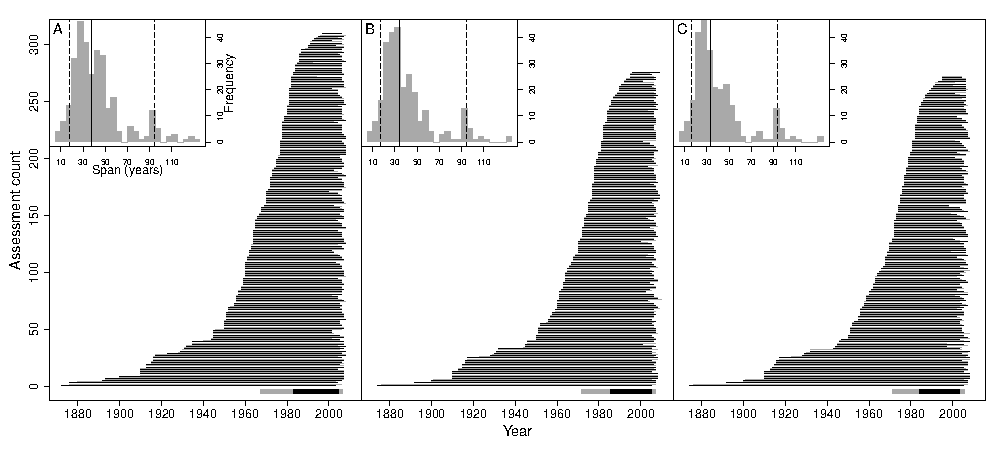
\includegraphics[width=8in]{/home/srdbadmin/srdb/projects/fishandfisheries/R/first-review/orca-plot.pdf}
\end{center}
\caption{ }\label{fig:orca}
\end{figure}
\end{landscape}

\begin{landscape}
\begin{figure}
\begin{center}
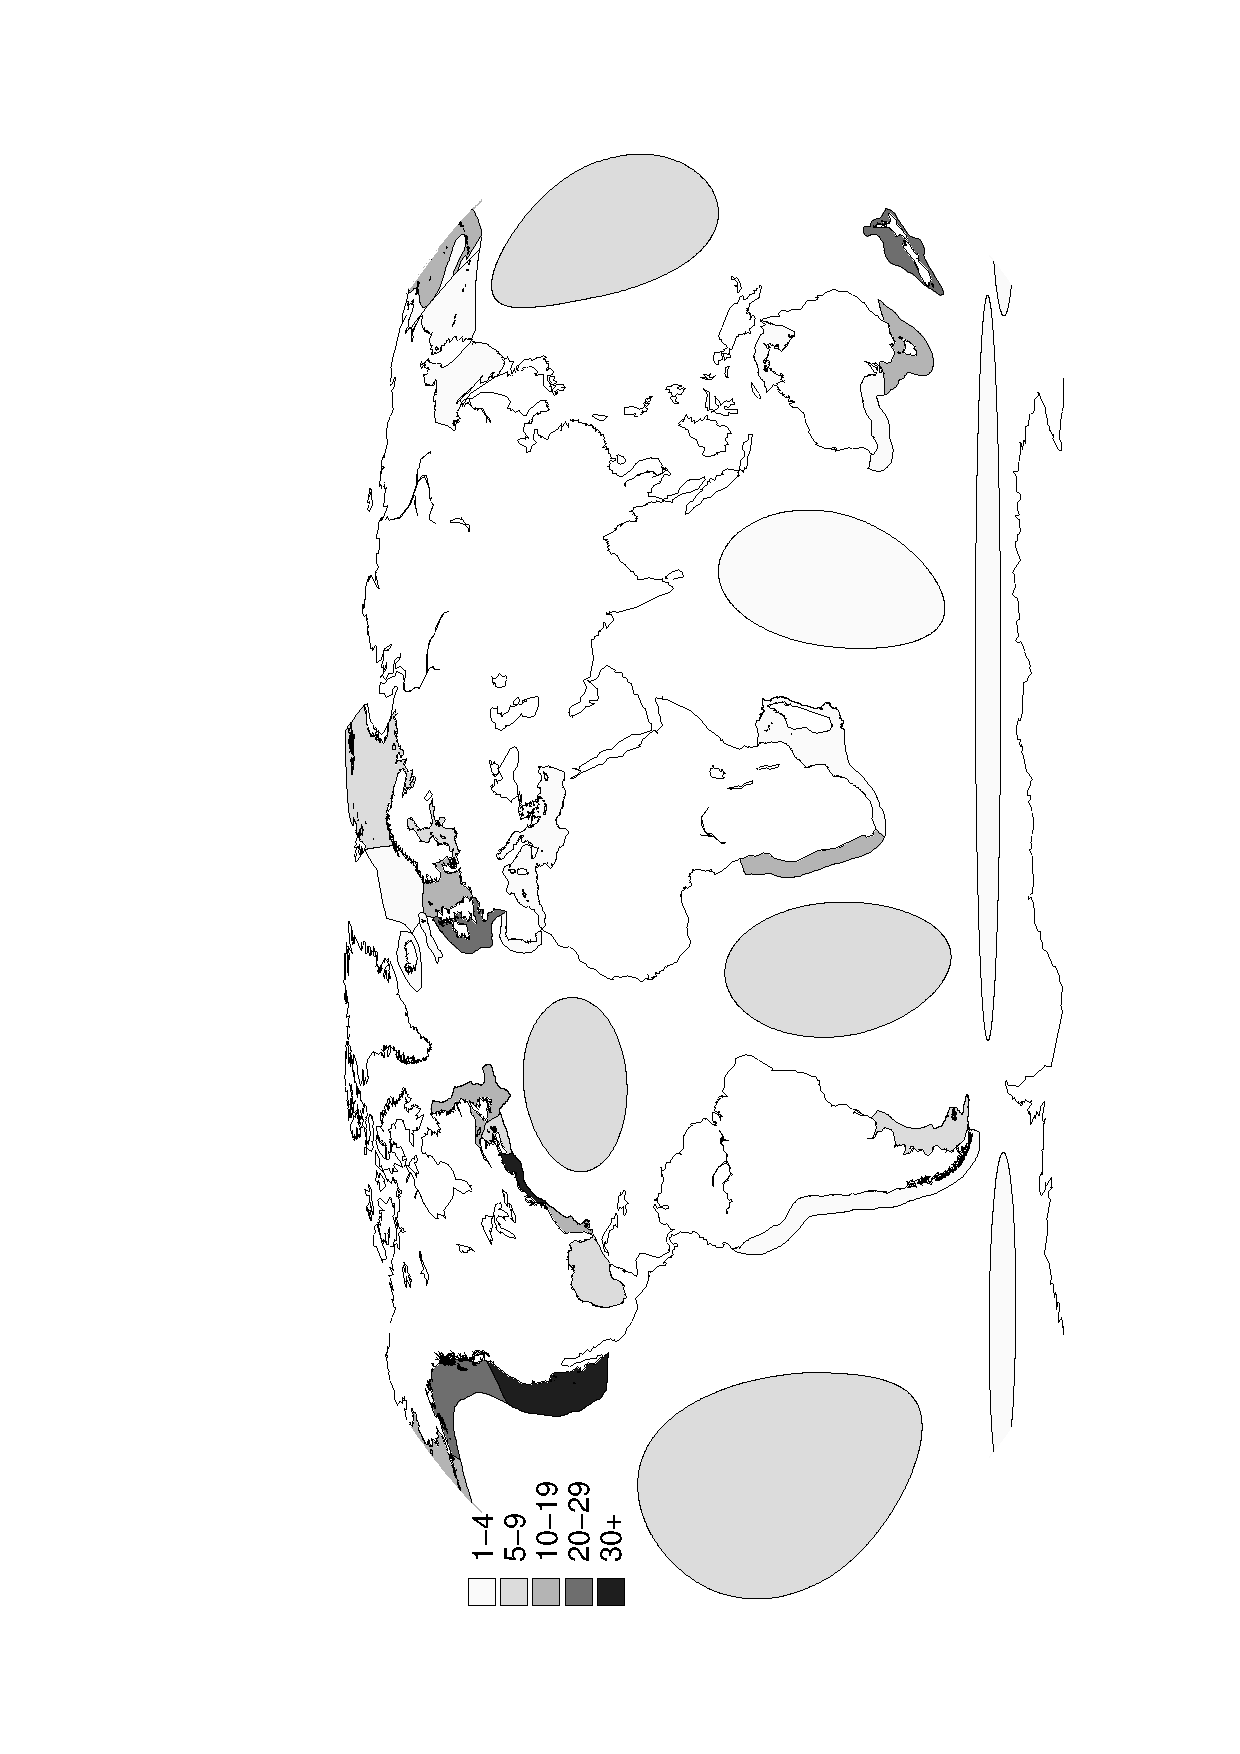
\includegraphics[width=9in]{/home/srdbadmin/srdb/projects/fishandfisheries/GMT/stocks-byLME.pdf}
\end{center}
\caption{ }\label{fig:lmes}
\end{figure}
\end{landscape}


\begin{figure}
\begin{center}
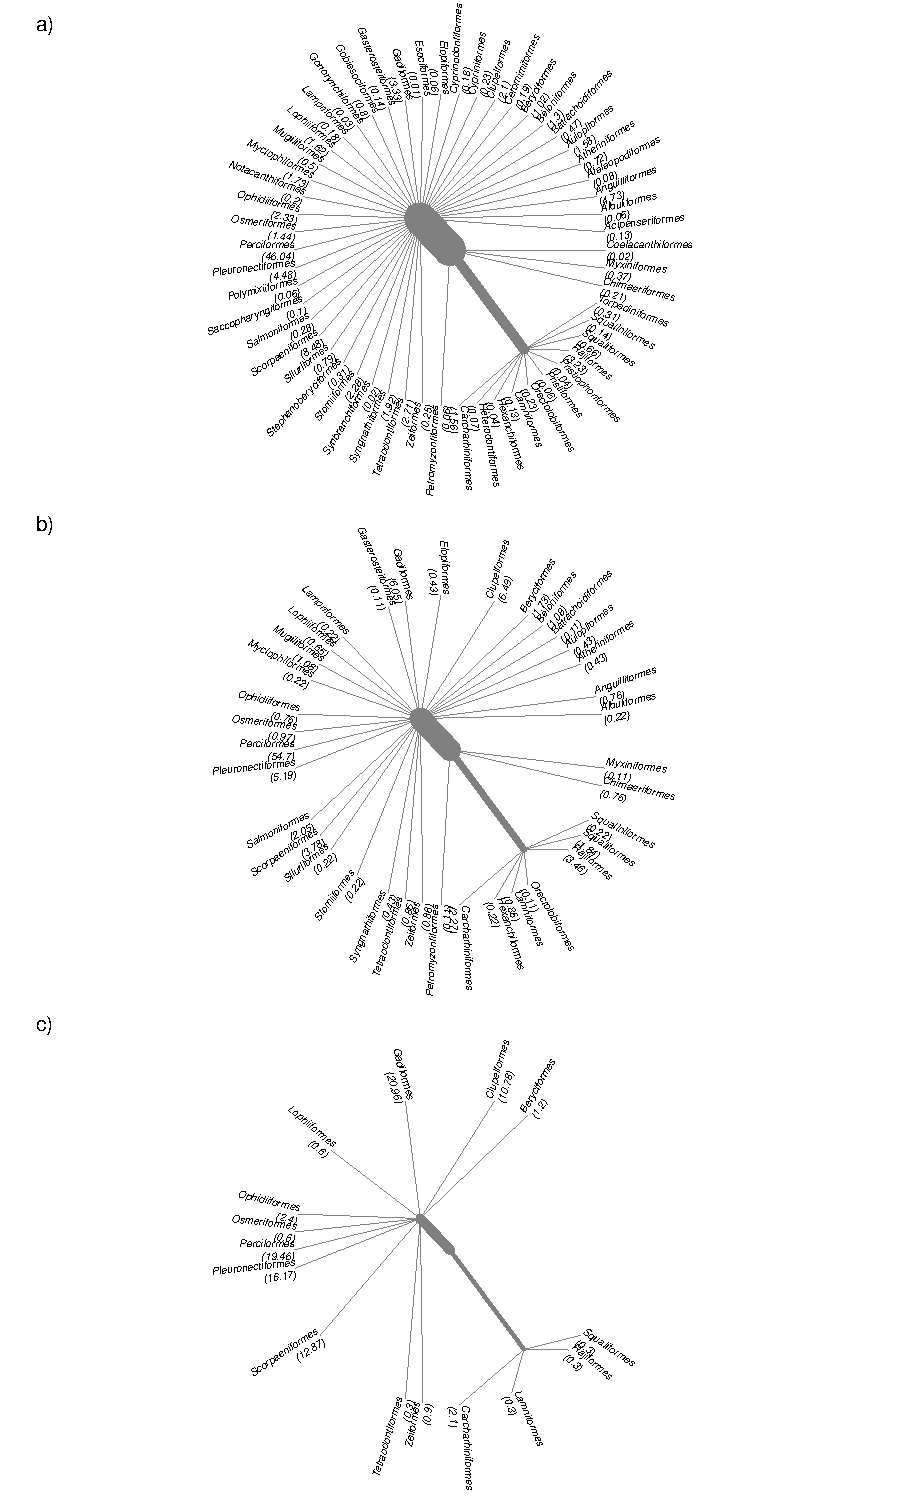
\includegraphics[height=8.5in]{/home/srdbadmin/srdb/projects/fishandfisheries/R/first-review/three-panel-phylo.pdf} % fishbase_saup_two_panel_phylo.pdf}
\end{center}
\caption{ }\label{fig:taxo:threepanel}
\end{figure}




%\begin{figure}
%\begin{center}
%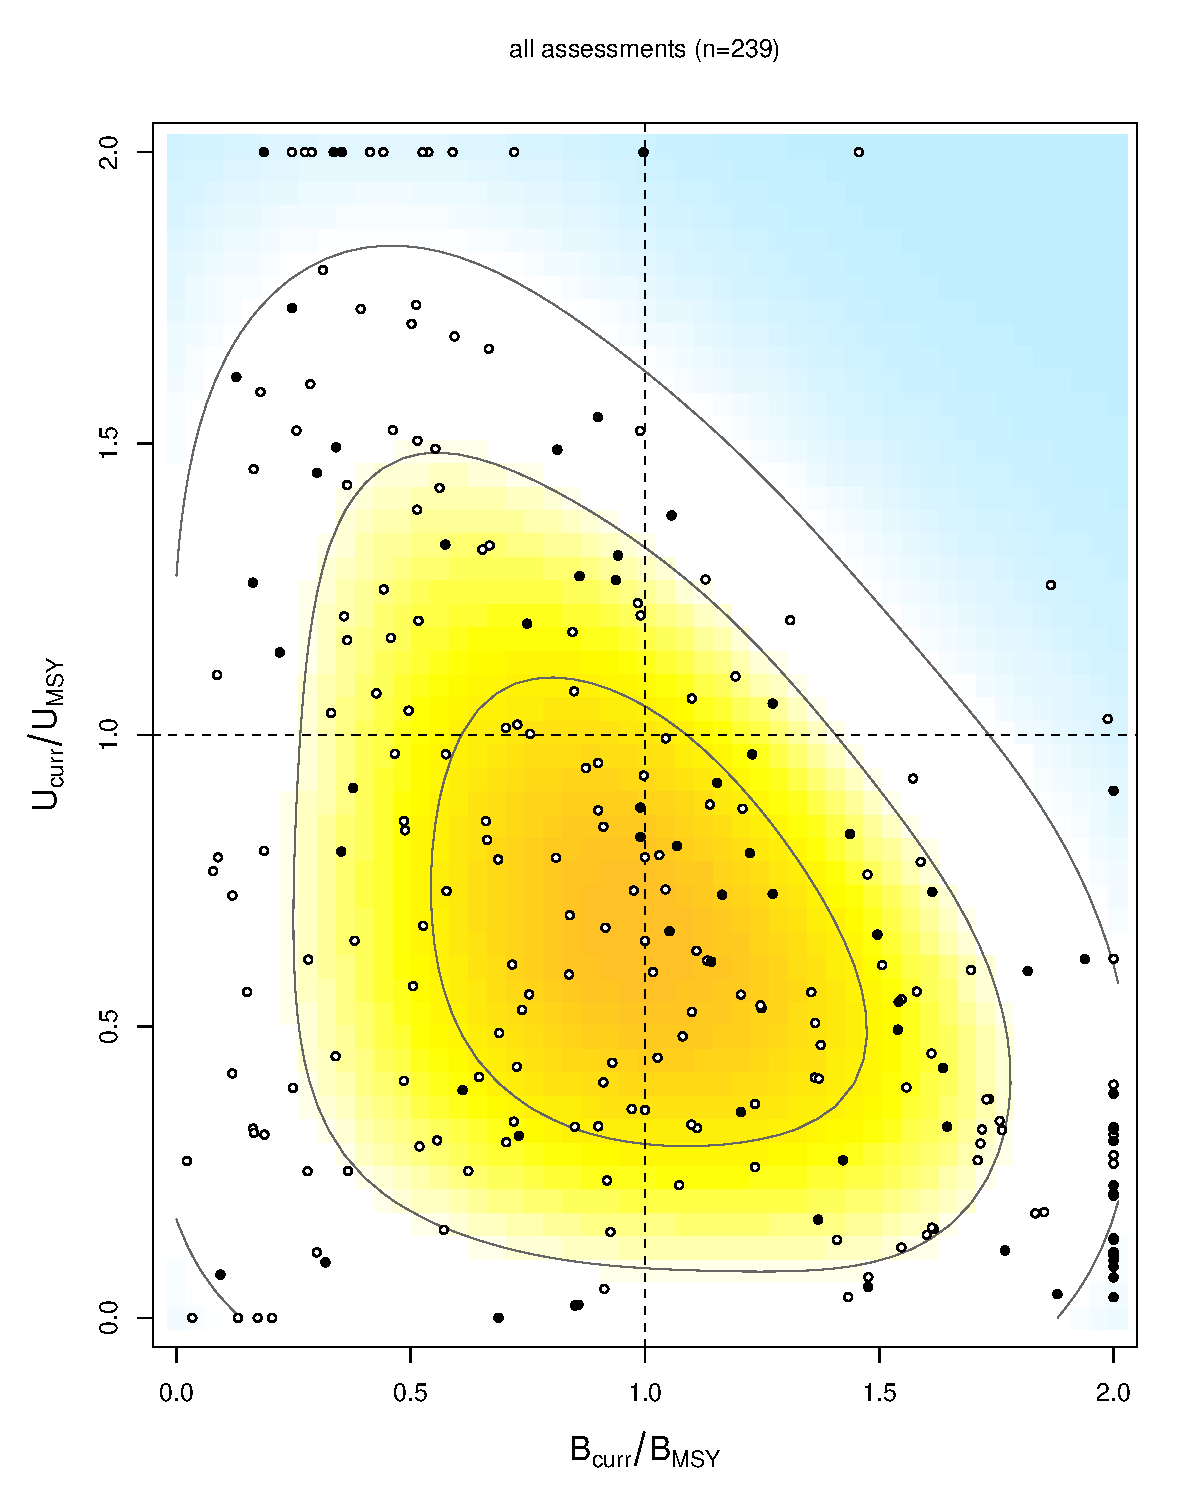
\includegraphics[width=15cm]{/home/srdbadmin/srdb/projects/fishandfisheries/R/first-review/friedegg-single.pdf}
%\end{center}
%\caption{ }\label{fig:friedegg}
%\end{figure}

%Some options for the management-level fried eggs.

%\begin{figure}
%\begin{center}
%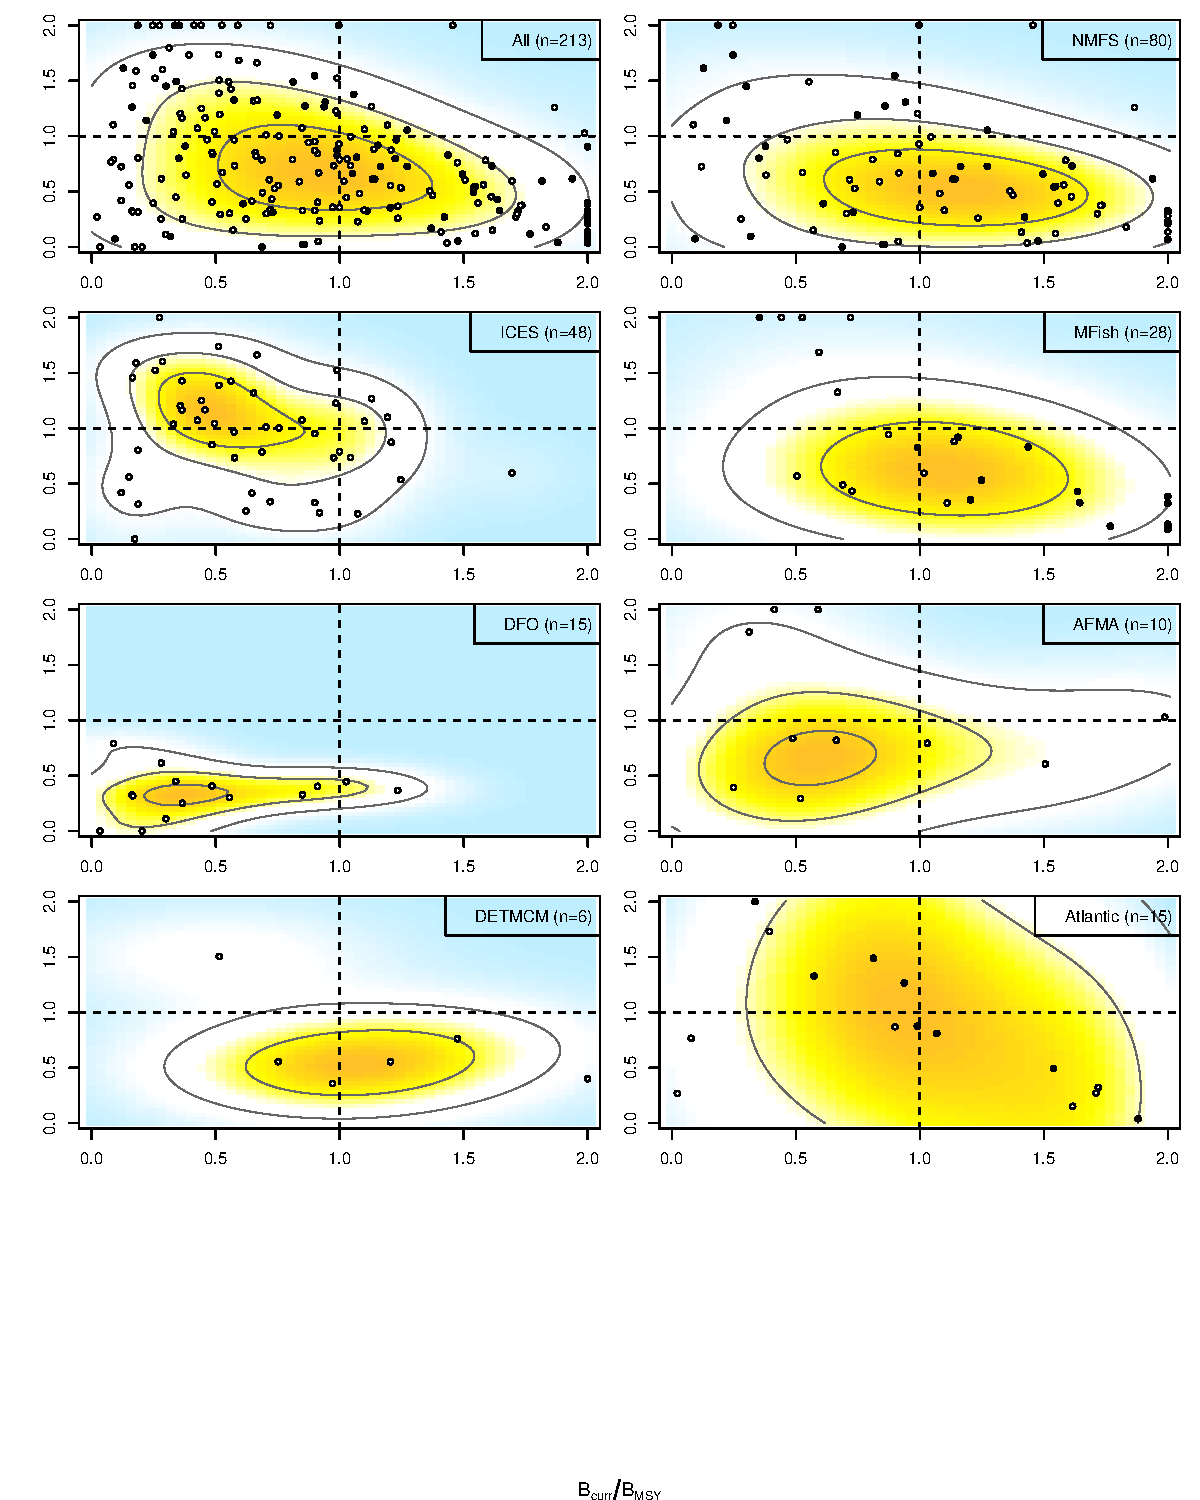
\includegraphics[width=15cm]{/home/srdbadmin/srdb/projects/fishandfisheries/R/first-review/friedegg-bymgmt.pdf}
%\end{center}
%\caption{Option 1 }\label{fig:friedegg}
%\end{figure}

%\begin{figure}
%\begin{center}
%\includegraphics[width=15cm]{/home/srdbadmin/srdb/projects/fishandfisheries/R/first-review/friedegg-bymgmt-10plots.pdf}
%\end{center}
%\caption{Option 2 }
%\end{figure}

\begin{landscape}
\begin{figure}
\begin{center}
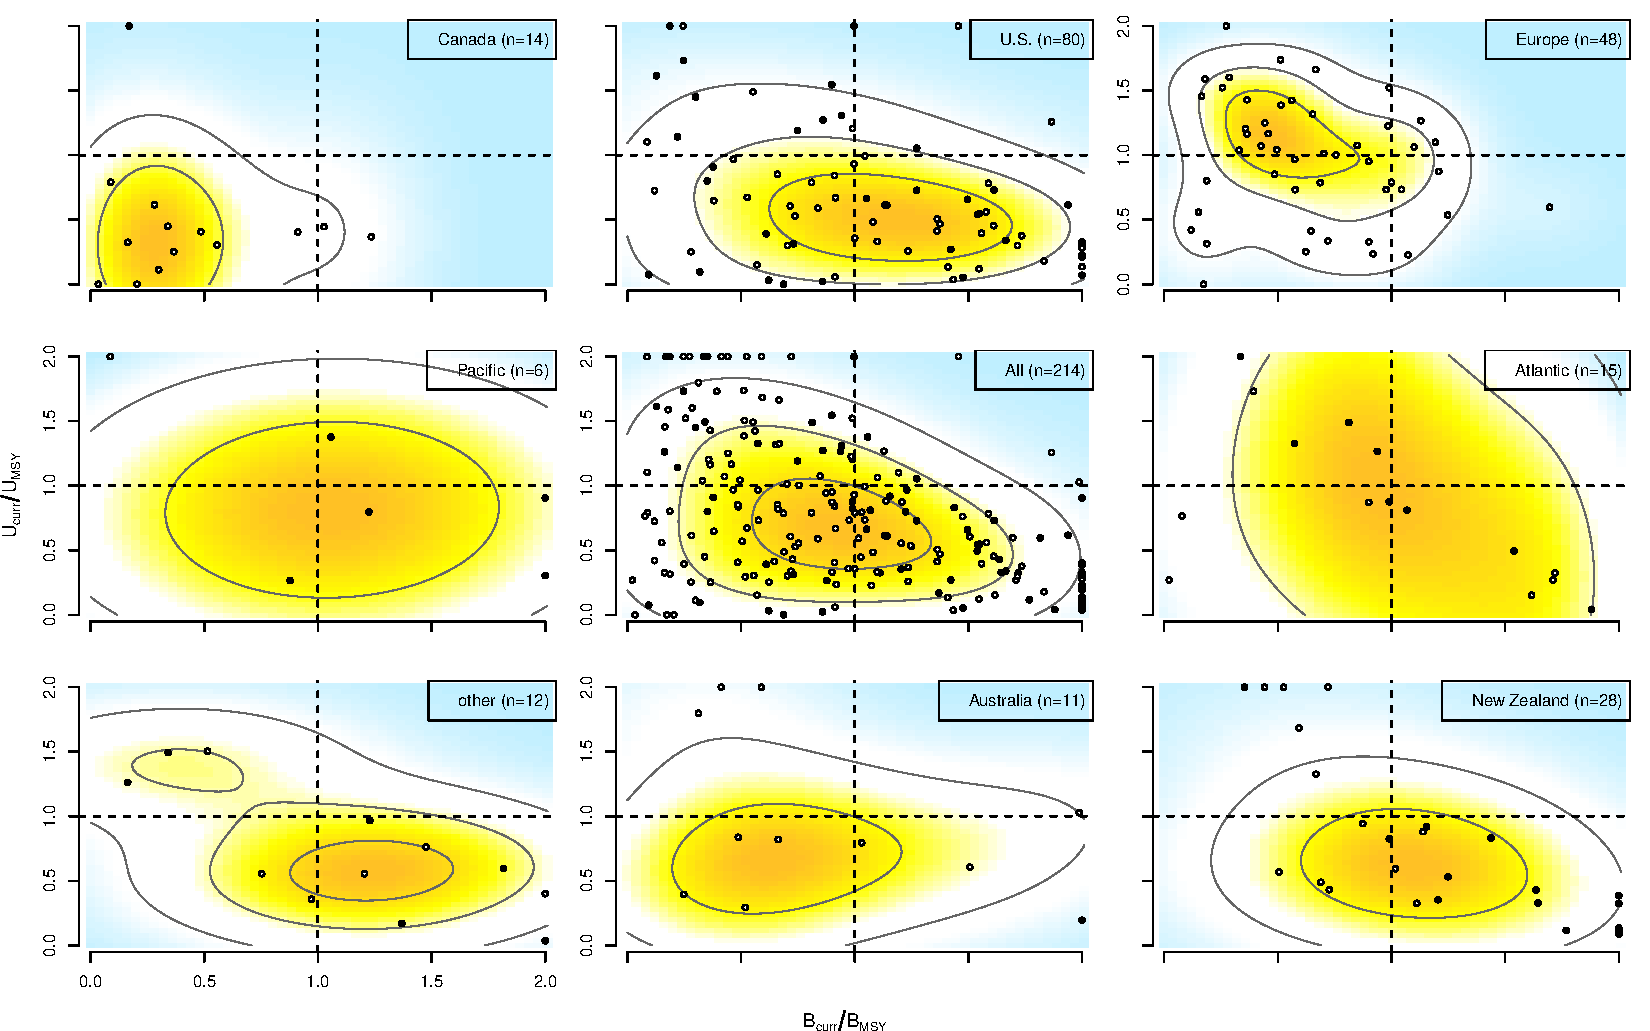
\includegraphics[width=9in]{/home/srdbadmin/srdb/projects/fishandfisheries/R/first-review/friedegg-9plots.pdf}
\end{center}
\caption{ Option 3}
\end{figure}
\end{landscape}

%For the top 6 taxonomic orders (Figure~\ref{fig:taxo}).
\begin{figure}
\begin{center}
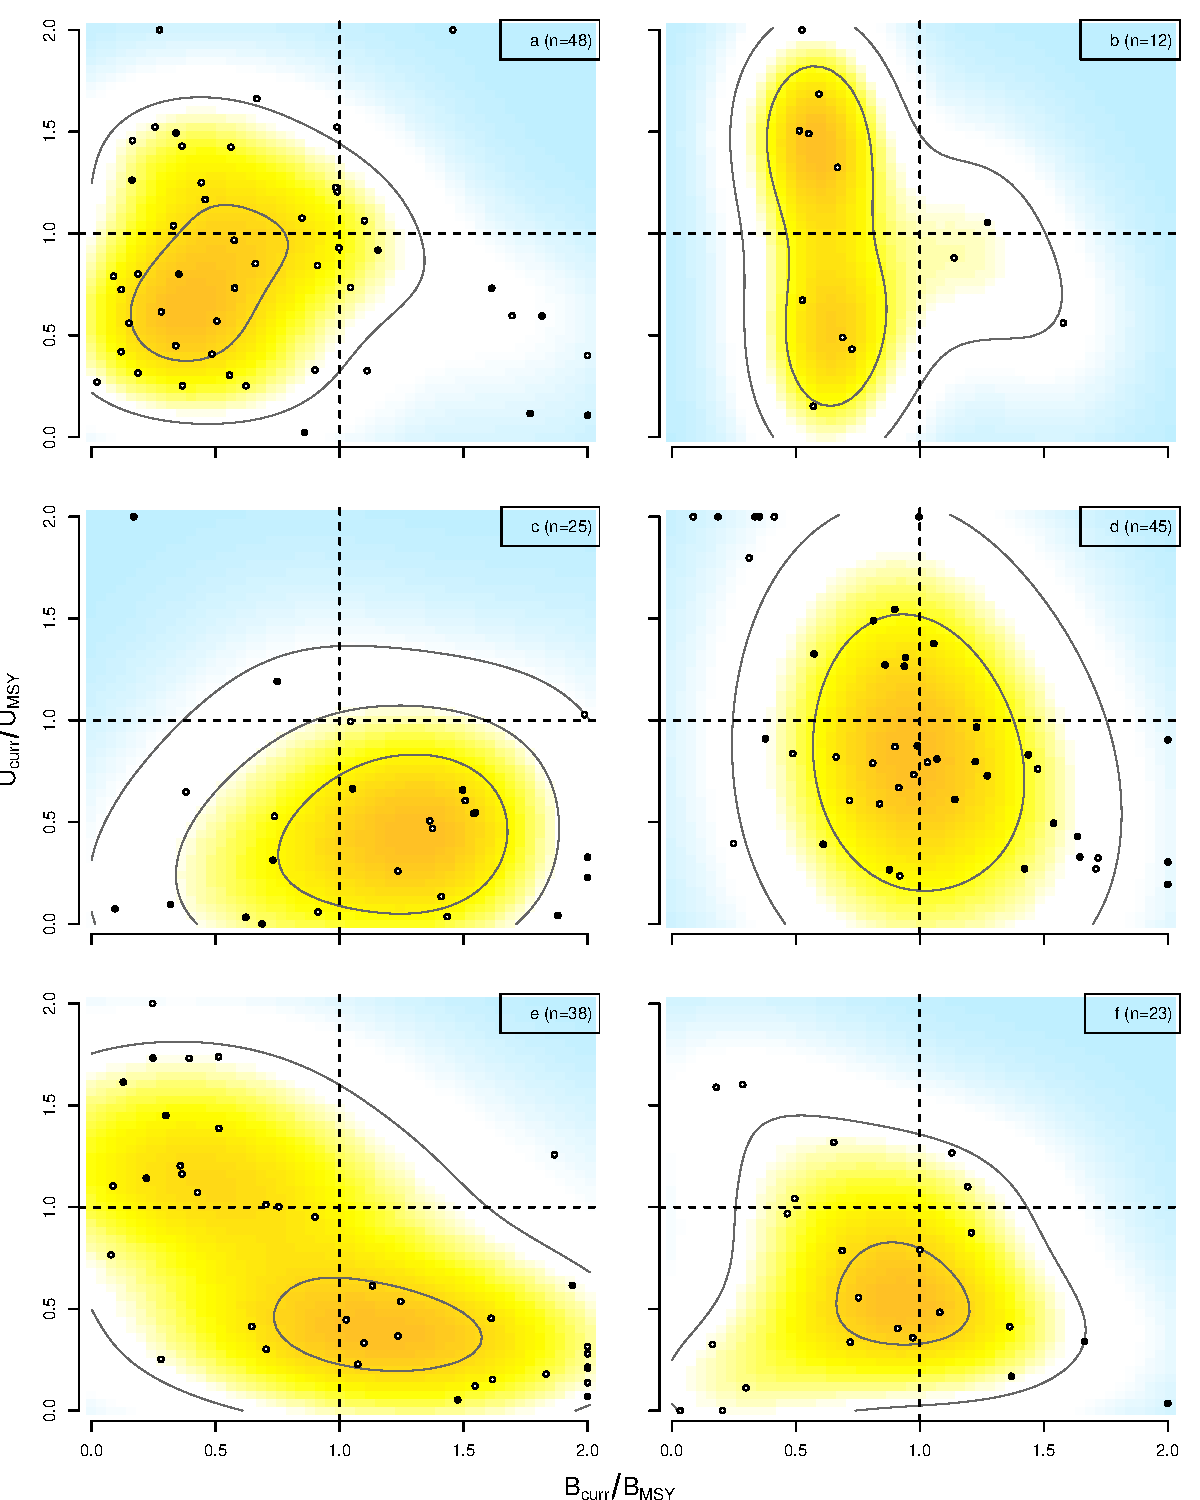
\includegraphics[width=15cm]{/home/srdbadmin/srdb/projects/fishandfisheries/R/first-review/friedegg-taxo.pdf}
\end{center}
\caption{Top 6 taxonomic orders. }
\label{fig:taxo}
\end{figure}

%By trophic level (Figure~\ref{fig:mtl}).
\begin{figure}
\begin{center}
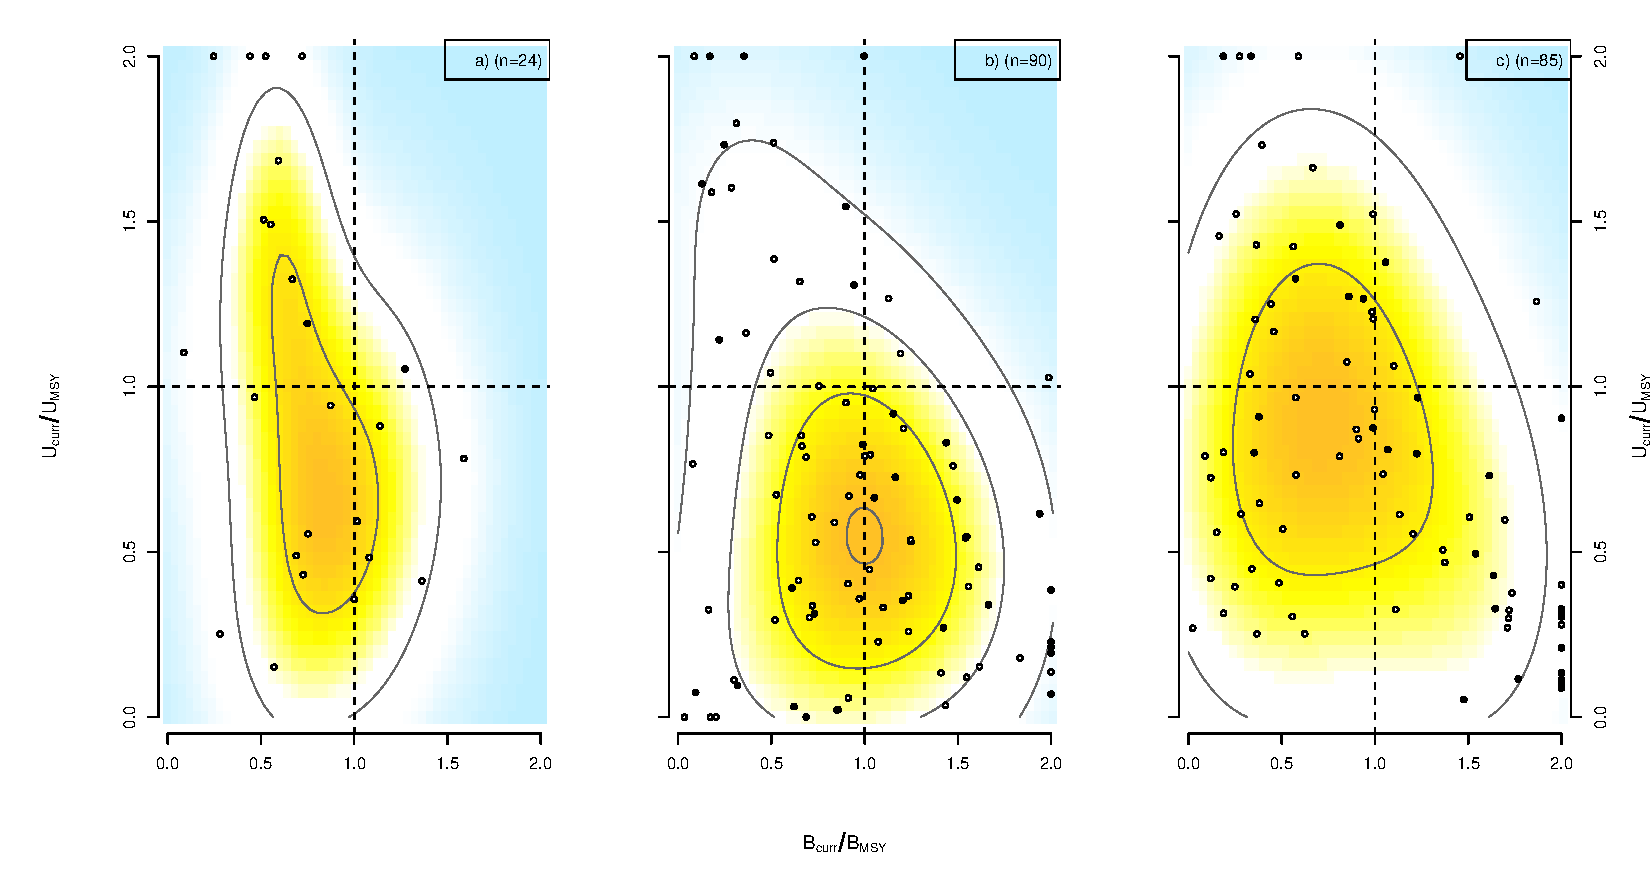
\includegraphics[width=15cm]{/home/srdbadmin/srdb/projects/fishandfisheries/R/first-review/friedegg-MTLs.pdf}
\end{center}
\caption{By mean trophic level (MTL).}
\label{fig:mtl}
\end{figure}







\end{document}

